\documentclass[12pt]{article}

\usepackage{amsmath}
\usepackage{amssymb}
\usepackage{calc}
\usepackage{units}
\usepackage{graphicx}
\usepackage[pdftex]{hyperref}
\usepackage{subfig}
\usepackage[margin=1in]{geometry}
\usepackage{listings}
\usepackage[numbers,sort&compress]{natbib}
\usepackage{bm}
\usepackage{paralist}
\usepackage[draft]{fixme}
\usepackage{textcomp}

\hypersetup{
  breaklinks=true,
  pdftitle={D.C. Circuits},
  pdfauthor={Kevin R. Lynch based on a lab by D.C.Jain}, 
  pdfsubject={Phyiscs, Electricity and magnetism},
  pdfkeywords={resistance, resistor, Ohm's Law},
  pdflang={en-US},
}

\title{D.C. Circuits}
\author{}
%Kevin R. Lynch, based on an earlier lab by D.C.Jain
%\date{2012-02-6}
\date{}

\begin{document}

\maketitle

\section{Objectives}
\label{sec:objectives}

\begin{enumerate}
\item To determine the resistance of resistors using
  \begin{inparaenum}
  \item a multimeter, and
  \item Ohm's Law,
  \end{inparaenum}
\item To verify the equivalent resistance formulae for series and
  parallel resistor combinations, and
\item To calculate voltage drop and current draw in series and
  parallel resistor combinations.
\end{enumerate}

\section{Introduction}
\label{sec:introduction}

According to Ohm's Law the electric current in an ohmic conductor is
directly proportional to the potential difference (or voltage drop)
between the ends of the conductor.  Thus, if $V$ is the potential
difference between the ends of the conductor, and the current through
the conductor is $I$, then
\begin{gather*}
  V = IR\ ,
\end{gather*}
where the constant of proportionality, $R$, is known as the
resistance.  The resistance of an Ohmic conductor depends mildly on
temperature.

The voltage drop across a resistor is caused by the dissipation of
power in the resistor itself.  Normally, this power dissipation
manifests as heat (known as ohmic heating).  The power dissipated is
the product of the voltage drop and the current draw
\begin{gather*}
  P = VI = I^2 R = \frac{V^2}{R}\ .
\end{gather*}

There is a certain maximum power draw, $P_\mathrm{max}$, that real
resistors can safely dissipate without an undue temperature rise, and
correspondingly, a maximum safe current, $I_\mathrm{max}$, which the
resistor can handle without overheating.  The previous equation gives
\begin{gather*}
  I_\mathrm{max} = \sqrt{\frac{P_\mathrm{max}}{R}}\ ,
\end{gather*}
where $P_\mathrm{max}$ is the maximum rated power.  Resistors used in
this laboratory have $P_\mathrm{max} = \unit[1]{W}$; resistors in
consumer electronics are typically rated for
$\unit[\nicefrac{1}{10}]{W}$ or less, while industrial power resistors
with multi-\unit{kW} ratings are also available.

\begin{figure}
  \centering
    \subfloat[][Axial lead]{
    \label{fig:resistors:axial}
    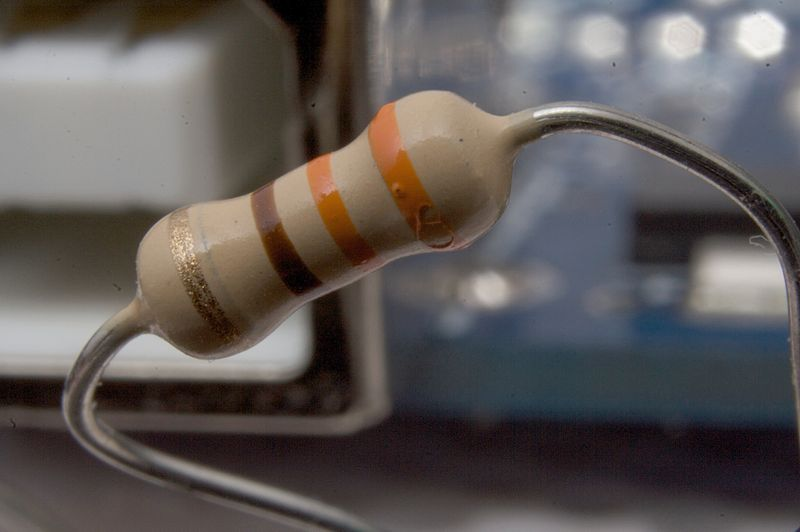
\includegraphics[width=\textwidth/3]{figures/Resistor}
%% Figure license under CCA-SA 3.0
%% http://en.wikipedia.org/wiki/File:Resistor.jpg
  } \qquad
  \subfloat[][Surface mount]{
    \label{fig:resistors:smd}
    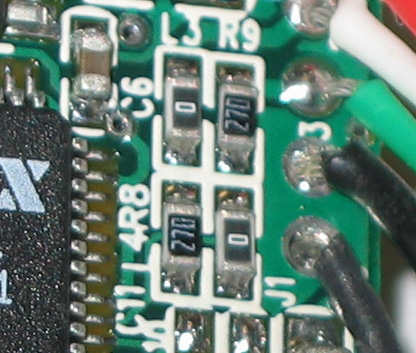
\includegraphics[width=\textwidth/3]{figures/Zero_ohm_resistors_cropped}
%% Figure license under CCA-SA 3.0
%% http://en.wikipedia.org/wiki/File:Zero_ohm_resistors_cropped.jpg
  }  
  \caption{The left hand figure shows a standard axial lead resistor
    (the resistor leads emerge along the axis, hence the name).  The
    color code is clearly visible (see Table~\ref{tab:colorcode}); the
    displayed resistor has a value of $\unit[330 \pm 5\%]{\Omega}$.
    The right hand figure shows modern ``surface mount device'', or
    SMD resistors.  They are \textit{not} color coded, but instead
    typically have a numerical value code written on them.  In this
    image, we see $\unit[0]{\Omega}$ (aka ``jumpers'') and two
    $\unit[27]{\Omega}$ resistors.}
  \label{fig:resistors}
\end{figure}
%%
\begin{table}
  \centering
  \subfloat[][Value Band Codes]{
    \begin{tabular}{|c|c|c|c|}\hline
      Band Color & Value & Band Color & Value\\ \hline 
      Black & 0 & Green & 5 \\
      Brown & 1 & Blue & 6 \\
      Red & 2 & Violet & 7 \\
      Orange & 3 & Gray & 8 \\
      Yellow & 4 & White & 9 \\ \hline
    \end{tabular}} \qquad
  \subfloat[][Common Tolerance Band Codes]{
    \begin{tabular}{|c|c|}\hline
      Band Color & Tolerance [\%]\\ \hline
      Brown & 1\\
      Red & 2\\
      Gold & 5\\
      Silver & 10\\
      None & 20\\ \hline
    \end{tabular}
  }
  \caption{The resistance value (in Ohms) of axial lead resistors are
    indicated directly on the resistor by a series of color coded
    bands (see Figure~\ref{fig:resistors:axial}).  The typical resistor
    code is a four or five band code, in a form that resembles
    scientific or engineering notation: for a resistor with $n$ bands,
    the first $n-2$ bands (starting with the band nearest a lead) are
    the mantissa, the $n-1$st band is the exponent, and the last band
    is the \textit{tolerance}.  A four band code gives $c_1 c_2 \times
    10^{c_3}\Omega \pm c_4\%$; for example, brown-brown-black-gold is
    $11\times10^{0}\Omega \pm 5\% = 11\Omega \pm 5\%$.  Resistors are
    not generally available in all possible combinations of values;
    you can't, for instance, buy a $50\Omega$ resistor of any
    tolerance, but you can buy a $49.9\Omega$ or a $51\Omega$ resistor.}
  \label{tab:colorcode}
\end{table}
The resistors we will use are the classic ``carbon composite axial
lead'' type; while particularly convenient for this lab, they are not
used much anymore, except in niche applications.  For modern consumer
or high precision electronics, however, they are both too inaccurate,
and too large to use.  The convenience factor for hands-on work is
great: they are large enough for you to measure and manipulate by
hand, they are labeled with a standard color banding code
(Table~\ref{tab:colorcode}) and they are easy to attach to a board via
hand soldering.

\section{Theory}
\label{sec:theory}

\begin{figure}
  \centering
    \subfloat[][Series]{
    \label{fig:combinations:series}
    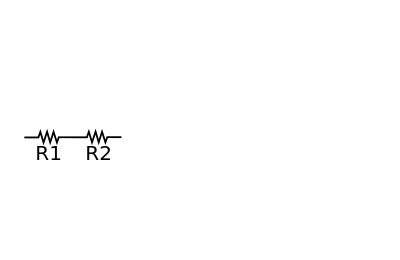
\includegraphics[width=\textwidth/3]{figures/series}
  } \qquad
  \subfloat[][Parallel]{
    \label{fig:combinations:parallel}
    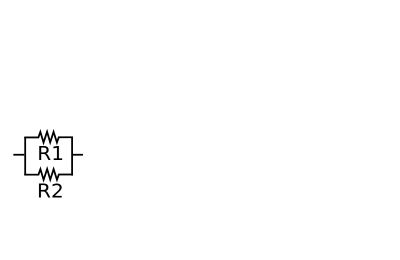
\includegraphics[width=\textwidth/3]{figures/parallel}
  }  
  \caption{Series and parallel resistor configurations.}
  \label{fig:combinations}
\end{figure}
When two or more resistors are connected in a circuit, they can always
be replaced with an \textit{equivalent resistor} that has the same
effect as the individual resistors.  In fact, from the point of view
of the power supply, which can only see the global properties of the
circuit (resistance, and a few others we will discuss later in the
semester), the entire circuit can be reduced to a single equivalent
resistance.  To perform these replacements, however, we must know the
rules to apply.  For series combined resistors, as shown in
Figure~\ref{fig:combinations:series}, the equivalent resistance is the
sum of all the individual resistances:
\begin{gather*}
  R_S = R_1 + R_2 + R_3 + \cdots = \sum_i R_i\ .
\end{gather*}
This is because the same current must pass through each resistor.  For
parallel combined resistors, as shown in
Figure~\ref{fig:combinations:parallel}, the inverse of the equivalent
resistance is the sum of the inverses of the individual resistances:
\begin{gather*}
  \frac{1}{R_P } = \frac{1}{R_1} + \frac{1}{R_2} + \frac{1}{R_3} +
  \cdots = \sum_i \frac{1}{R_i}\ .
\end{gather*}
In this case, the voltage drop across all of the resistors must be the
same, so the total current is divided between all the resistors
according to Ohm's Law.  The current in a given \textit{branch} of the
parallel circuit is inversely proportional to the resistance of that
branch.

\begin{figure}
  \centering
  \includegraphics[width=2\textwidth/3]{figures/circuit}
  \caption{The circuit used to test the parallel and series resistance
    combinations.} 
  \label{fig:circuit}
\end{figure}
More complicated combinations of resistors can often be reduced to
``nested'' collections of parallel and series resistances.  For
instance, in the circuit in Figure~\ref{fig:circuit}, the effective
resistance of all five resistors can be determined first by combining
the three parallel resistors $R_3$, $R_4$, and $R_5$, into a single
effective resistance $R_P$, and then combining the three series
resistors $R_1$, $R_2$, and $R_P$ into a single effective resistance
$R_S$.

\section{Procedures}
\label{sec:procedures}

In this lab, we will work with premounted, \unit[1]{W} resistors, a
power supply, and a pair of multimeters.  

\begin{enumerate}
\item Choose five resistors from the board and find their resistances
  and tolerances using the color code described in
  Table~\ref{tab:colorcode}.
\item Configure one of the multimeters to measure resistance, then
  measure the resistances of the five resistors you chose in the
  previous step by using the meter.  Are the measured values within
  the stated tolerances?
\item Calculate the maximum safe current for each resistor,
  $I_{i,\mathrm{max}}$; the current in each resistor must be kept
  below this maximum safe value.  In later steps, you must make sure
  that the power supply does not drive more than the maximum safe
  current through any of the resistors.
\item Build the circuit shown in Figure~\ref{fig:circuit}.  In this
  experiment, the ammeter has two purposes:
  \begin{inparaenum}
  \item To ensure that the current remains constant throughout the
    measurements, and
  \item To ensure that you don't exceed the maximum safe current
    through any resistor.
  \end{inparaenum}
\item Determine a safe operating voltage for this circuit.  Calculate
  the maximum safe voltage using Ohm's Law and the series and parallel
  resistance formulae.  Set the power supply voltage below this value,
  and then check (by touching!) each connected resistor to make sure
  it isn't getting hot!
\item Set the second multimeter to read DC Voltage.  Measure and
  record the potential difference across the power supply.  Then,
  measure the potential difference across each of the resistors.
\item Next, set the second multimeter to read DC Current.  Measure and
  record the current passing through each of the five resistors.  You
  should make sure that the current passing through the first ammeter
  stays constant throughout your measurements!
\item Remove the meters and power supply from the circuit.  Measure
  and record the resistance between the following sets of points:
  $AD$, $AC$, $BD$, and $CD$.  You've already measured the values of
  the individual resistors; do your measurements of the parallel and
  series combinations match with predictions?
\end{enumerate}

\newpage

\section*{Pre-Lab Exercises}

Answer these questions as instructed on Blackboard; make sure to
submit them before your lab session!

\begin{enumerate}
\item What is the safe operating voltage for a $\unit[100]{\Omega}$,
  \unit[\nicefrac{1}{10}]{W} resistor?  The maximum current?  How much
  power is dissipated at half the maximum voltage?
\item What is the resistance of an ideal voltmeter?  Do you connect a
  voltmeter in series or parallel with the potential drop you are
  trying to measure?
\item What is the resistance of an ideal ammeter?  Do you connect an
  ammeter in series or parallel with the current draw you are trying
  to measure?
\item Write an expression for the equivalent resistance of three
  parallel resistors.  What about three series resistors?
\item If a resistor is banded Red-Blue-Green-Silver, what are the
  minimum and maximum resistance values in the tolerance range?
\end{enumerate}

\newpage

\section*{Post-Lab Exercises}

\begin{enumerate}
\item For the five resistors in your measurement, tabulate the
  following data:
  \begin{inparaenum}
  \item the nominal resistance given by the color code,
  \item the nominal tolerance,
  \item the direct multimeter measurement of their values,
  \item the percent difference between the nominal and measured
    resistance, and
  \item the maximum safe current.
  \end{inparaenum}
  How did you define the percent difference? Are all of the measured
  values equal to the nominal values within tolerance?
\item Tabulate the voltage drop across, and current through, each of
  your resistors.  From these data, derive the resistance of each
  resistor.  Do these derived values match the directly measured
  values in your first table?
\item In the last step of the procedure, you measured a number of
  different series and parallel combinations of resistors.  Using the
  individual measured resistor values, predict these combinations.  Do
  your predictions match the measurements?  Why or why not?
\item The voltage drops around a closed loop must equal zero.  The
  circuit studied here forms a closed loop; the power supply
  \textit{raises} the voltage, while the voltage drops around the
  circuit reduce the voltage.  Do these sum to zero in this
  experiment?  Why or why not?
\item Due to charge conservation, the current leaving the positive
  terminal of the power supply must return to the negative terminal.
  Does your circuit satisfy these requirements?  How can you tell?
\item Energy conservation demands that the power delivered to the
  circuit by the power supply must equal the power dissipated in the
  circuit.  Tabulate the total power delivered and the power
  dissipated in each resistor.  Are they equal?
\item Discuss briefly whether you have met the objectives of the lab
  exercises.
\end{enumerate}

\end{document}

%%% Local Variables: 
%%% mode: latex
%%% TeX-master: t
%%% End: 
